
\begin{figure*}[t]
    \centering

    \begin{subfigure}[b]{.23\linewidth}
        \centering
        \includegraphics[width=\linewidth]{figure/plot/reference/fig10a-covert-inode-pmem.tikz.pdf}
        \caption{[Ref] NVRAM}
        \label{fig:10:ref:covert-inode-nvram}
    \end{subfigure}
    \hfill
    \begin{subfigure}[b]{.23\linewidth}
        \centering
        \includegraphics[width=\linewidth]{figure/plot/reference/fig10b-covert-inode-dram.tikz.pdf}
        \caption{[Ref] DRAM}
        \label{fig:10:ref:covert-inode-dram}
    \end{subfigure}
    \hfill
    \begin{subfigure}[b]{.23\linewidth}
        \centering
        \resizebox{\linewidth}{!}{\includegraphics{example-image-duck}}
        % \includegraphics[width=\linewidth]{figure/plot/reproduce/fig10a-covert-inode-pmem.tikz.pdf}
        \caption{[Rep] NVRAM}
        \label{fig:10:rep:covert-inode-nvram}
    \end{subfigure}
    \hfill
    \begin{subfigure}[b]{.23\linewidth}
        \centering
        \resizebox{\linewidth}{!}{\includegraphics{example-image-duck}}
        % \includegraphics[width=\linewidth]{figure/plot/reproduce/fig10b-covert-inode-dram.tikz.pdf}
        \caption{[Rep] DRAM}
        \label{fig:10:rep:covert-inode-dram}
    \end{subfigure}

    \caption{Filesystem inode-based covert channel on NVRAM and DRAM.}
    \label{fig:10:covert-inode}
\end{figure*}
